\documentclass[../Main.tex]{subfiles}
\begin{document}
\chapter{Data Analytics}

\intro{
    Data Analytics is the process of examining, cleaning, transforming, and 
    modelling data to extract useful insights, support decision-making, and 
    identify patterns. 
    It involves cleaning, transforming, and modelling data using statistical 
    analysis, machine learning, and data visualization to interpret complex 
    datasets. 
    Businesses, researchers, and organisations use data analytics to optimise 
    performance, predict trends, and drive strategic decisions.
}

\defn{Datenkompetenz (Data Literacy)}{
Umfasst die Fähigkeiten, Daten auf kritische Art und Weise zu sammeln, zu 
managen, zu bewerten und anzuwenden.

Grundlegende Fragen:
    \begin{enumerate}
        \item Was will ich mit Daten machen?
        \item Was kann ich mit Daten machen?
        \item Was darf ich mit Daten machen?
        \item Was soll ich mit Daten machn?
    \end{enumerate}
}

\section{Datentypen und Skalenniveaus}
Die Bestimmung der Datenmerkmale ermöglicht es erst, Daten zu 
organisieren, zu analysieren und schliesslich zu nutzen.
Das führt zu Skalenniveaus (Attributs-Merkmals-Levels, en: "Levels of 
measurement" or "Scales of measure")

\begin{figure}[H]
    \centering
    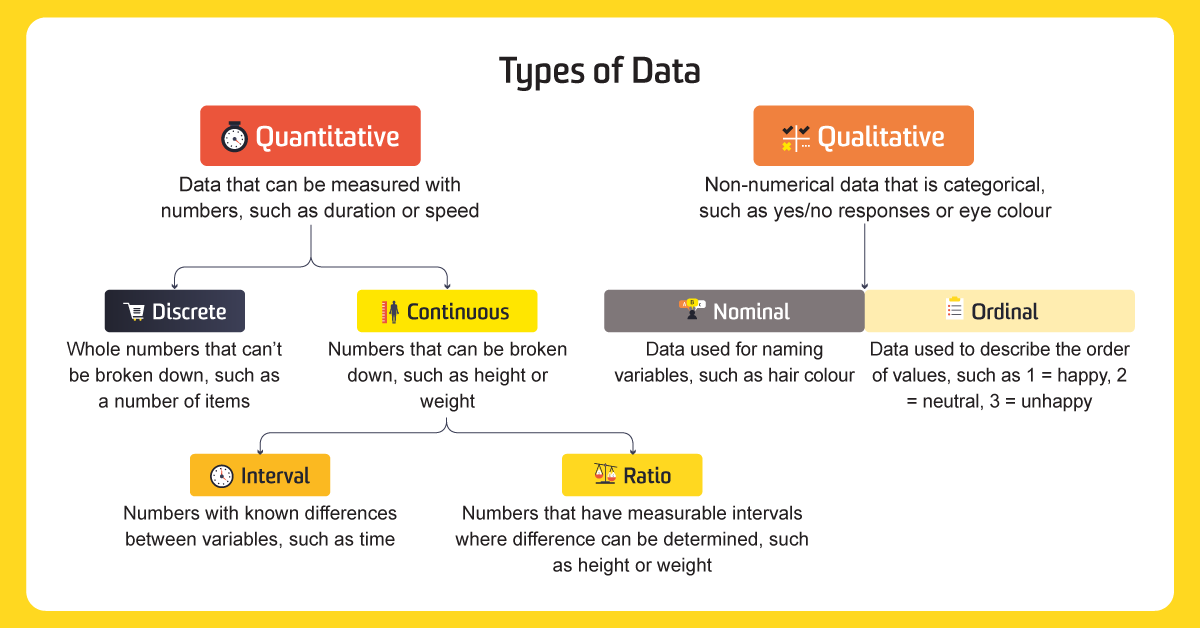
\includegraphics[width=0.75\linewidth]{Images/datentypen.png}
    \caption{Datentypen}
\end{figure}


\begin{multicols}{2}
    \defn{Qualitative Daten}{
        \begin{itemize}
            \item Beziehen sich auf Informationen die nicht gemessen werden
            \item In der Regel beschreibend also in Textform (können auch numerisch codiert sein).
        \end{itemize}
    }
    \defn{Quantitative Daten}{
        \begin{itemize}
            \item Werden verwendet, um Informationen zu definieren, die gezählt werden können. 
            \item Sind numerisch.
        \end{itemize}
    }
\end{multicols}

\defn{NOIR}{
    \begin{itemize}
        \item Nominalskala
        \item Ordinalskala
        \item Intervallskala
        \item Verhältnisskala (Ratio)
    \end{itemize}
}

\begin{figure}[H]
    \centering
    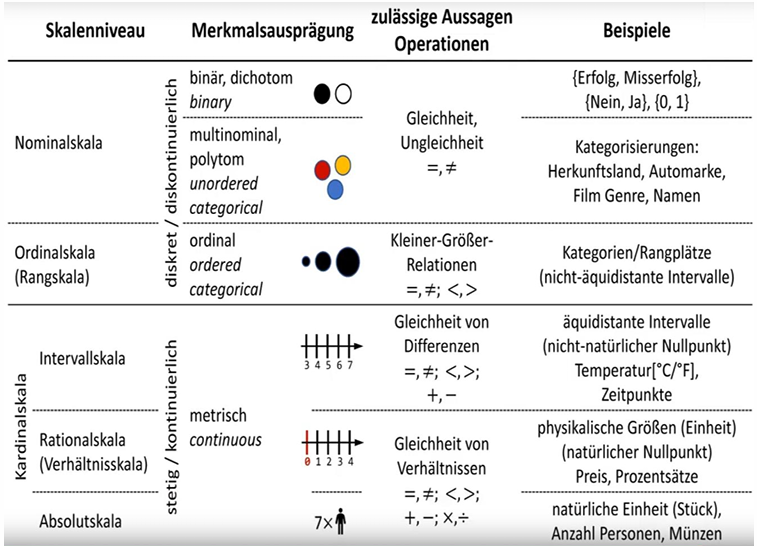
\includegraphics[width=0.75\linewidth]{Images/noir.png}
    \caption{NOIR}
\end{figure}

\section{Business Intelligence (BI)}
Datenvisualisierungs- und –Publikation-Werkzeuge ist allgemeiner  
und auch kurz Business Intelligence-Werkzeug (BI Tools) genannt.
Früher sprach man auch von Decision Support Systems.

\begin{multicols}{2}
    \defn{BI Tools}{
        Sind Tools und Technologien, die Unternehmen einsetzen, um Daten zu sammeln, zu 
        analysieren und in aussagekräftige Erkenntnisse und Wissen umzuwandeln, das für 
        fundierte Geschäftsentscheidungen genutzt werden kann. Umfasst den Einsatz von 
        Analyse, Data Mining, Data Warehousing und Reporting.
    }
    \defn{Decision Support Systems (DSS)}{
        Sind computergestützte Informationssysteme mit Methoden, die Entscheidungsträgern 
        helfen, bessere und fundiertere Entscheidungen zu treffen (bezüglich Ist-Zustand, 
        zurückblickenden Analyse).

        Dabei gibt es verschiedene Ansätze:
        \begin{itemize}
            \item Datenbankansatz (inkl. Visualisierung)
            \item Data-Mining-Ansatz
            \item Informationsbeschaffungsansatz
        \end{itemize}
    }
    BI liefert die Daten und Erkenntnisse, die für die Entscheidungsfindung erforderlich sind, 
    während DSS die Werkzeuge und Methoden für diese Entscheidungen bereitstellt.
\end{multicols}

Die wohl verbreitetsten Produkte sind die kommerziellen Anwendungen:
\begin{itemize}
    \item Tableau
    \item Ms Power BI
\end{itemize}
Weitere Produkte:
\begin{itemize}
    \item Looker
    \item Apache Superset
    \item Oracle Analytics
    \item Datawrapper
\end{itemize}


\begin{figure}[H]
    \centering
    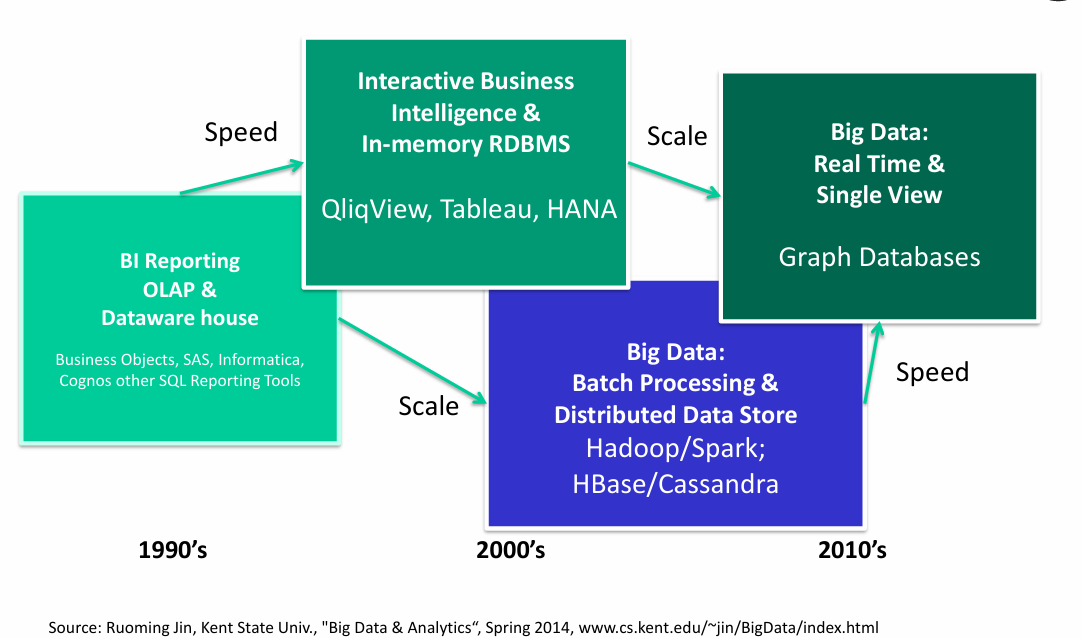
\includegraphics[width=0.75\linewidth]{Images/evolutionbi.png}
    \caption{Evolution of BI}
\end{figure}

\defn{7 Types of Quantitative Messages}{
    \begin{itemize}
        \item Nominal Comparison
        \item Time-Series
        \item Part-to-Whole
        \item Deviation
        \item Frequency distribution
        \item Correlation
    \end{itemize}
    Stephen Few
}

\begin{figure}[H]
    \centering
    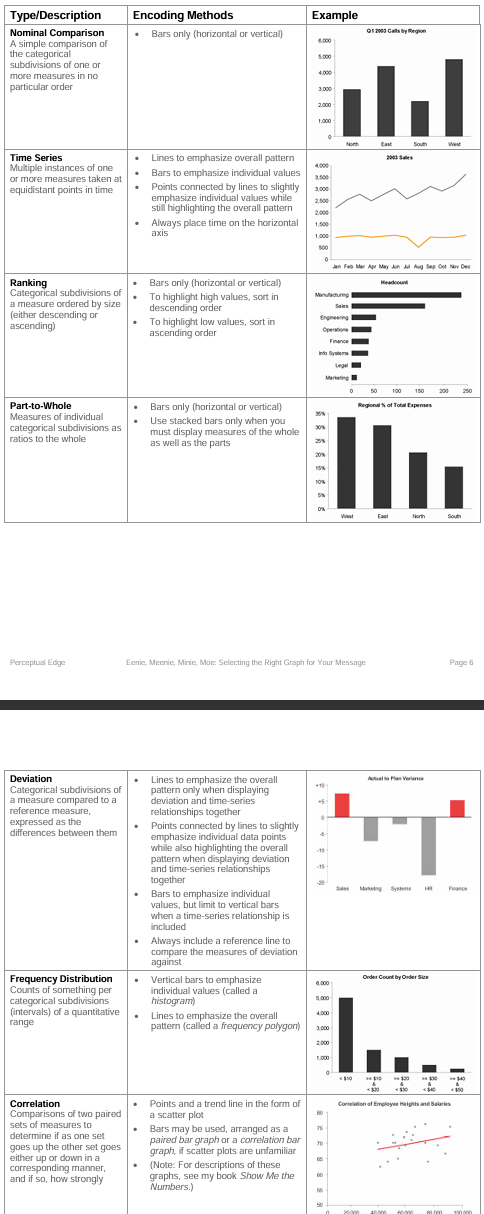
\includegraphics[width=0.5\linewidth]{Images/quantitative-messages.png}
    \caption{Quantitative Messages}
\end{figure}

\defn{Graphical Integrity by Tufte}{
    \begin{enumerate}
        \item The representation of numbers, as physically 
        measured on the surface of the graph itself, 
        should be directly proportional to the 
        numerical quantities represented.
        \item Clear, detailed and thorough labeling should 
        be used to defeat graphical distortion and 
        ambiguity. Write out explanations of the data 
        on the graph itself. Label important events in 
        the data.
        \item Show data variation, not design variation.
        \item In time-series displays of money, 
        deflated and standardized units of 
        monetary measurement are nearly 
        always better than nominal units.
        ("Deflating" means adjusting for inflation,
        so the values reflect purchasing power rather
        than just raw monetary amounts.)
        \item  The number of information carrying 
        (variable) dimensions depicted 
        should not exceed the number of 
        dimensions in the data.
        Graphics must not quote data out of context.
    \end{enumerate}
}

\defn{Data Ink Principles by Tufte}{
    \begin{enumerate}
        \item Above all else show data.
        \item Maximize the data-ink ratio.
        \item Erase non-data-ink.
        \item Erase redundant data-ink.
        \item Revise and edit
    \end{enumerate}
    The data-ink ratio is calculated by 1 minus the proportion of the graph 
    that can be erased without loss of data-information.
}


\begin{figure}[H]
    \centering
    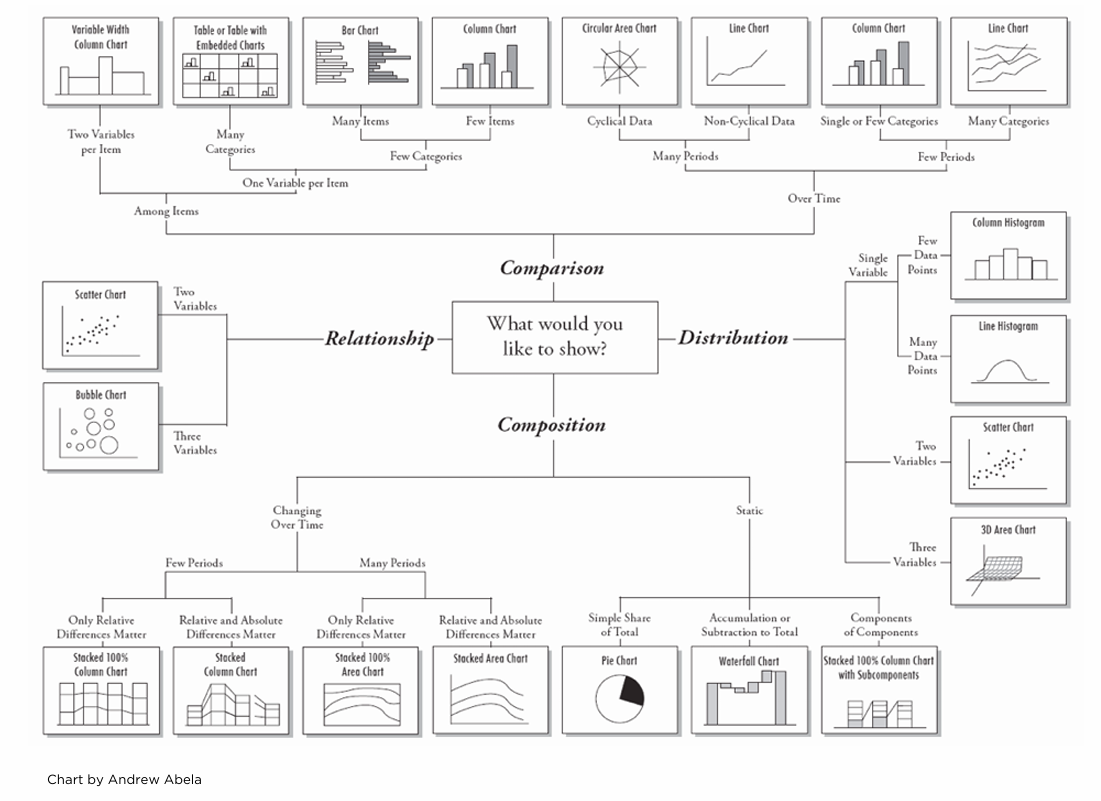
\includegraphics[width=1\linewidth]{Images/visualization-guideline.png}
    \caption{Visualization Guideline by Abela}
\end{figure}

\href{https://en.wikipedia.org/wiki/Visual_variable}{Visual Variable (Wikipedia)}

\end{document}
